\documentclass{webofc}
\usepackage[varg]{txfonts}
\usepackage{graphicx}
\usepackage{minted}

% 6 pages excluding references!

\begin{document}
\title{Awkward Arrays in Python, C++, and Numba}

\author{%
\firstname{Jim} \lastname{Pivarski}\inst{1}\fnsep\thanks{\email{pivarski@princeton.edu}} \and
\firstname{Peter} \lastname{Elmer}\inst{1}\fnsep\thanks{\email{Peter.Elmer@cern.ch}} \and
\firstname{David} \lastname{Lange}\inst{1}\fnsep\thanks{\email{David.Lange@cern.ch}}}

\institute{Princeton University}

\abstract{%
  Insert your english abstract here.
}

\maketitle

\section{Introduction}

Columnar data structures, in which identically typed data fields are contiguous in memory, are a good fit to physics analysis use-cases. This was recognized as early as 1989 when columnwise ntuples were added to PAW and 1995 when ROOT's file format allowed for ``split'' objects. In the past decade, with the Google Dremel paper [ref], the Parquet file format [ref], the Arrow memory interchange format [ref], and the inclusion of ``ragged tensors'' in TensorFlow [ref], the significance of hierarchical columnar data structures has been recognized beyond particle physics.

With the exception of the Columnar Objects experiment of T.\ Mattis et.\ al.\ [ref] and the XND library [ref], all of these projects focus on representing, storing, and transmitting columnar data structures, rather than operating on them. Physicists need to apply structure-changing transformations to search for decay topology candidates and other tasks that can change the level of nesting and multiplicity of their data. Operations of this complexity can be defined in terms of a suite of primitives.

The Awkward Array library [2018 ROOT workshop ref] was created to fill this need (not addressed by XND's current scope) with hooks to transform Awkward Arrays to and from ROOT, Arrow, and others, without copying in some cases. Since its release in September 2018, this library has become one of the most widely pip-installed packages for particle physics (see Figure~\ref{fig:pip-timeline}).

\begin{figure}
\begin{center}
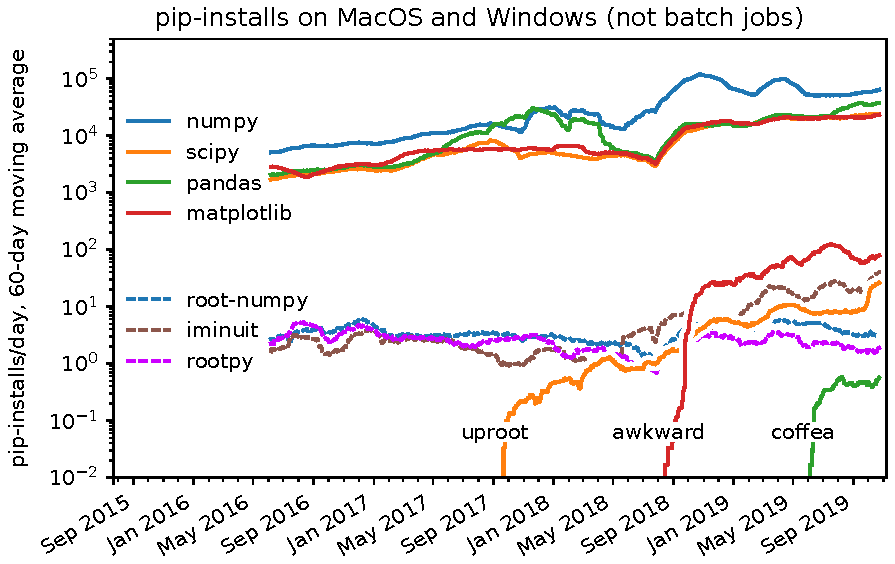
\includegraphics[width=0.75\linewidth]{pip-timeline.pdf}
\end{center}
\caption{Number of pip-installations per day (smoothed by a 60-day moving average) for popular data analysis libraries (numpy, scipy, pandas, matplotlib) and particle physics libraries (root-numpy, iminuit, rootpy, uproot, awkward, coffea) on operating systems not used for batch jobs. \label{fig:pip-timeline}}
\end{figure}

Feedback from physicists, such as the interviews we reported [2019 ACAT paper ref] and private conversations following a series of tutorials, has revealed that physicists appreciate the array-at-a-time operations when it's easy to see how an analysis task can be expressed with them, but would additionally like imperative access. The original class/method structure has led to some confusion and naming conflicts, and the composable structures that provide flexibility should be hidden from data-focused analyzers. Additionally, the original implementation in pure NumPy has led to maintainance issues---all of these argue for a reimplementation of the Awkward Array concept with a better architecture and interface.

\section{Architecture}

\subsection{High-level Python layer}

\subsection{C++ layer}

\subsection{Numba layer}

\subsection{Kernels layer}

\section{Record-oriented $\to$ columnar}

% \subsection{Deeply nested data from ROOT}

\section{Status}

\section{Conclusion}




%% \section{Introduction}
%% \label{intro}
%% Your text comes here. Separate text sections with

%% \section{Section title}
%% \label{sec-1}
%% For bibliography use \cite{RefJ}

%% % BibTeX or Biber users please use (the style is already called in the class, ensure that the "woc.bst" style is in your local directory)
%% % \bibliography{name or your bibliography database}
%% %
%% % Non-BibTeX users please use
%% \begin{thebibliography}{}
%% % and use \bibitem to create references.
%% \bibitem{RefJ}
%% Journal Author, Journal \textbf{Volume}, page numbers (year)
%% \end{thebibliography}

\end{document}
